\begin{pastexam}[label={px:ntu-110-esoe-ds-07}]{臺大工科海洋所 110 學年度（A）第 7 題}
（問答）

\textbf{(15 \%)} For the graph as shown:
\begin{enumerate}[label=(\alph*)]
\item (8 \%) Give the adjacency matrix representation.
\item (7 \%) Draw the minimum spanning tree.
\end{enumerate}
\begin{center}
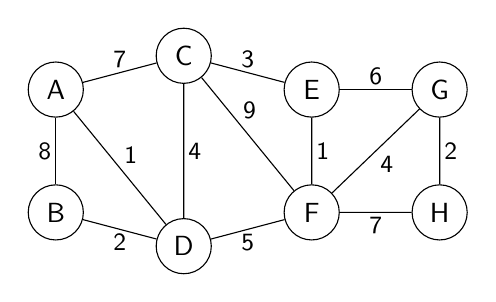
\begin{tikzpicture}[scale=1.3,v/.style={circle,draw,inner sep=1pt,minimum size=7mm,font=\sffamily},l/.style={inner sep=1.5pt,font=\small\sffamily}]
\node[v] (A) at (0,0) {A}; \node[v] (C) at (1.25,0.33) {C}; \node[v] (E) at (2.5,0) {E}; \node[v] (G) at (3.75,0) {G};
\node[v] (B) at (0,-1.2) {B}; \node[v] (D) at (1.25,-1.53) {D}; \node[v] (F) at (2.5,-1.2) {F}; \node[v] (H) at (3.75,-1.2) {H};
\draw (A) -- node[l,above] {7} (C);
\draw (C) -- node[l,above] {3} (E);
\draw (E) -- node[l,above] {6} (G);
\draw (A) -- node[l,left] {8} (B);
\draw (A) -- node[l,above right] {1} (D);
\draw (C) -- node[l,right] {4} (D);
\draw (C) -- node[l,pos=0.4,above right] {9} (F);
\draw (E) -- node[l,right] {1} (F);
\draw (G) -- node[l,below right] {4} (F);
\draw (G) -- node[l,right] {2} (H);
\draw (B) -- node[l,below] {2} (D);
\draw (D) -- node[l,below] {5} (F);
\draw (F) -- node[l,below] {7} (H);
\end{tikzpicture}
\end{center}
\end{pastexam}

\begin{pastsoln}
圖有 $8$ 個頂點、$13$ 條無向加權邊：$AB\,8$、$AC\,7$、$AD\,1$、$BD\,2$、$CD\,4$、$CE\,3$、$CF\,9$、$DF\,5$、
$EF\,1$、$EG\,6$、$FG\,4$、$FH\,7$、$GH\,2$。

\textbf{(a)} 加權圖的相鄰矩陣 $W$：$W[i][j]$ 是邊 $\{i, j\}$ 的權重，沒有邊記 $\infty$，對角線記 $0$
（資結書第~21.2~節）。 無向圖的矩陣是對稱的。
\begin{center}
\begin{tabular}{c|*{8}{c}}
 & A & B & C & D & E & F & G & H \\
\hline
A & 0 & 8 & 7 & 1 & $\infty$ & $\infty$ & $\infty$ & $\infty$ \\
B & 8 & 0 & $\infty$ & 2 & $\infty$ & $\infty$ & $\infty$ & $\infty$ \\
C & 7 & $\infty$ & 0 & 4 & 3 & 9 & $\infty$ & $\infty$ \\
D & 1 & 2 & 4 & 0 & $\infty$ & 5 & $\infty$ & $\infty$ \\
E & $\infty$ & $\infty$ & 3 & $\infty$ & 0 & 1 & 6 & $\infty$ \\
F & $\infty$ & $\infty$ & 9 & 5 & 1 & 0 & 4 & 7 \\
G & $\infty$ & $\infty$ & $\infty$ & $\infty$ & 6 & 4 & 0 & 2 \\
H & $\infty$ & $\infty$ & $\infty$ & $\infty$ & $\infty$ & 7 & 2 & 0 \\
\end{tabular}
\end{center}
有的課本沒有邊時記 $0$，那是因為權重都是正的、不會和真正的邊混淆；寫的時候說明清楚即可。 只要
表示「有沒有邊」的話，把每個數字換成 $1$、$\infty$ 換成 $0$。

\textbf{(b)} 用 Kruskal（資結書第~24.2~節）：邊依權重由小到大，兩端不在同一棵樹就加入，在同一棵樹
（會形成環）就跳過。 權重相同的邊依字母順序。
\begin{center}
\begin{tabular}{clll}
\toprule
邊 & 權重 & 動作 & 加入後的元件 \\
\midrule
$AD$ & 1 & 加入 & $\{A, D\}$ \\
$EF$ & 1 & 加入 & $\{A, D\}, \{E, F\}$ \\
$BD$ & 2 & 加入 & $\{A, B, D\}, \{E, F\}$ \\
$GH$ & 2 & 加入 & $\{A, B, D\}, \{E, F\}, \{G, H\}$ \\
$CE$ & 3 & 加入 & $\{A, B, D\}, \{C, E, F\}, \{G, H\}$ \\
$CD$ & 4 & 加入 & $\{A, B, C, D, E, F\}, \{G, H\}$ \\
$FG$ & 4 & 加入 & 全部 8 個頂點 \\
\bottomrule
\end{tabular}
\end{center}
已經有 $7 = 8 - 1$ 條邊，停止；後面的 $DF\,5$、$EG\,6$、$AC\,7$、$FH\,7$、$AB\,8$、$CF\,9$ 兩端都已經
相連，都會形成環。 最小生成樹的邊是 $AD, EF, BD, GH, CE, CD, FG$，總權重 $1 + 1 + 2 + 2 + 3 + 4 + 4 = 17$。
\begin{center}
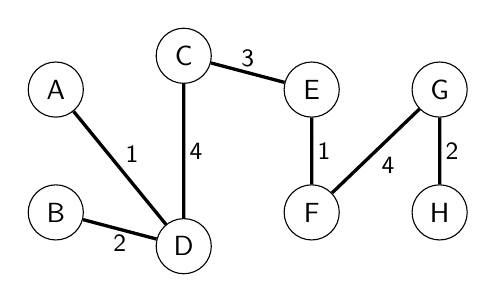
\begin{tikzpicture}[scale=1.3,v/.style={circle,draw,inner sep=1pt,minimum size=7mm,font=\sffamily},l/.style={inner sep=1.5pt,font=\small\sffamily}]
\node[v] (A) at (0,0) {A}; \node[v] (C) at (1.25,0.33) {C}; \node[v] (E) at (2.5,0) {E}; \node[v] (G) at (3.75,0) {G};
\node[v] (B) at (0,-1.2) {B}; \node[v] (D) at (1.25,-1.53) {D}; \node[v] (F) at (2.5,-1.2) {F}; \node[v] (H) at (3.75,-1.2) {H};
\draw[very thick] (C) -- node[l,above] {3} (E);
\draw[very thick] (A) -- node[l,above right] {1} (D);
\draw[very thick] (C) -- node[l,right] {4} (D);
\draw[very thick] (E) -- node[l,right] {1} (F);
\draw[very thick] (G) -- node[l,below right] {4} (F);
\draw[very thick] (G) -- node[l,right] {2} (H);
\draw[very thick] (B) -- node[l,below] {2} (D);
\end{tikzpicture}
\end{center}

\textbf{這棵是唯一的最小生成樹。} 對每條沒選的邊，看它和樹上路徑形成的環：$DF\,5$ 的環上其他邊是
$DC\,4, CE\,3, EF\,1$；$EG\,6$ 的是 $EF\,1, FG\,4$；$AC\,7$ 的是 $AD\,1, DC\,4$；$FH\,7$ 的是 $FG\,4, GH\,2$；
$AB\,8$ 的是 $AD\,1, DB\,2$；$CF\,9$ 的是 $CE\,3, EF\,1$。 每條沒選的邊都比它的環上其他邊重，所以都
不可能出現在任何最小生成樹裡（資結書第~24.1~節的環性質），答案唯一。 權重相同的 $CD$、$FG$ 誰先
處理都一樣，兩條都會加入。 用 Prim 從任何頂點開始也會得到同一棵樹。
\end{pastsoln}
